\documentclass[a4paper]{article}

\usepackage{times}
\usepackage{tikz}
\usepackage[margin=0cm]{geometry}
\usepackage{graphicx}
\usepackage{anyfontsize}
\usepackage{fancyhdr}
\usepackage{indentfirst}
\usepackage{amsmath}
\usepackage[spanish]{babel}
\usepackage[utf8]{inputenc}
\usepackage{titlesec}
\usepackage{enumitem}

\author{}
\date{}
\title{}

\begin{document}
\thispagestyle{empty}

\begin{tikzpicture}[remember picture, overlay]
    \pgftransformshift{\pgfpoint{0cm}{0cm}}
    \draw [line width=2pt](1cm,-1cm) -- (1cm,-27.7cm) -- (14cm, -27.7cm) -- (14cm, -1cm) -- (1cm, -1cm);
    \draw[line width=2pt] (15cm, -27.7cm) -- (19cm,-27.7cm) -- (19cm, -1cm) -- (15cm, -1cm) --  (15cm, -27.7cm);
    \node [line width=2pt] at (17cm, -3.5cm) {
\includegraphics[width=3cm]{../utn.png}};
		\node [line width=2pt] at (7.5cm, -7.5cm) {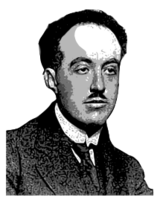
\includegraphics[width=6cm]{../broglie.png}};
    \node at (17cm, -7cm) {\scalebox{5}{\textbf{U}}};
    \node at (17cm, -9cm) {\scalebox{5}{\textbf{T}}};
    \node at (17cm, -11cm) {\scalebox{5}{\textbf{N}}};
    \node at (17cm, -14cm) {\scalebox{5}{\textbf{F}}};
    \node at (17cm, -16cm) {\scalebox{5}{\textbf{R}}};
    \node at (17cm, -18cm) {\scalebox{5}{\textbf{C}}};
    \node at (7.5cm, -12cm) {\scalebox{2.5}{\textbf{Longitud de onda}}};
    \node at (7.5cm, -13cm) {\scalebox{2.5} {\textbf{de \textit{DeBroglie}}}};

    \node at (7.5cm, -23cm) {
        \begin{minipage}[c]{12cm}
            \begin{itemize}
                \raggedright
                \vspace{1.5cm}
                \item \fontsize{12}{12}\selectfont \textbf{Autores:} \vspace {1mm} \fontsize{11}{12}\selectfont \\
                    \hspace{2mm} Valentino Rao - Leg. 402308 \\
                    \hspace{2mm} Ignacio Ismael Perea - Leg. 406265 \\
                    \hspace{2mm} Manuel Leon Parfait - Leg. 406599 \\ 
                    \hspace{2mm} Gonzalo Filsinger - Leg. 400460 \\ 
                    \hspace{2mm} Agustín Coronel - Leg. 402010 \\
                    \hspace{2mm} Marcos Raúl Gatica - Leg. 402006 \\

                \item \fontsize{12}{12}\selectfont \textbf{Curso:} 2R1. \\
                \item \fontsize{12}{12}\selectfont \textbf{Asignatura:} Física electrónica. \\
                \item \fontsize{12}{12}\selectfont \textbf{Institución:} Universidad Tecnológica Nacional - Facultad Regional de Córdoba \\

            \end{itemize}
        \end{minipage}};

\end{tikzpicture}

\renewcommand{\normalsize}{\fontsize{12}{18}\selectfont}
\newgeometry{margin=1cm}
\fancyhf{}
\renewcommand{\headrulewidth}{0pt}
\renewcommand{\footrulewidth}{0pt}
\fancyfoot[R]{[Rao V. - Parfait M. - Filsinger G. - Coronel A - Gatica M.] [\textbf{pág. \thepage}]}
\setlength{\footskip}{0pt}
\newpage
\thispagestyle{empty}
\text{}

\titleformat{\section} {\fontsize{12}{12}\bfseries}{\thesection.}{0.5em}{\underline}

\newpage
\newpage

\thispagestyle{empty}
\setcounter{page}{0}
\tableofcontents

\newpage
\thispagestyle{fancy}
\twocolumn
\flushbottom

\section{INTRODUCCIÓN}

    \indent El siguiente informe busca introducir el concepto de \textit{Ondas de DeBroglie} y el analísis de sus características corpusculares y de onda.

    \subsection{El principio de dualidad}
        \indent Con el descubrimiento de las propiedades corpusculares de las ondas en 1905, surge la hipótesis de que las partículas se comportan como tal aunque no exista una base experimental firme que la respalde. Esto último logró aportar \textit{Louis de Broglie en 1924}. \\
        
    \subsection{Las ondas de \textit{DeBroglie}}
        \indent Las ondas de \textit{DeBroglie} son aquellas cuya longitud de onda puede ser descripta por: \\

        \begin{center}
            $\lambda = \frac {h} {p}$ \\
        \end{center}
        
        \indent Siendo: \\
        \begin{itemize} [itemsep = -1.5em, topsep = 0em, leftmargin = 1cm]
            \item $\lambda$ = longitud de onda asociada a la partícula. \\
            \item \textit{h} = constante de Planck. \\
            \item \textit{p} = momento lineal de la partícula. \\
        \end{itemize}

        \indent Esto describe el comportamiento ondulatorio de las partículas según la teoría de la dualidad onda-partícula. \\

        \indent La demostración de este descriptor parte de conocer la longitud de onda de un fotón de luz: \\

        \begin{equation}
            p = \frac {hv} {c} \tag*{\textit{Momento del fotón.}}  \\
        \end{equation}

        \begin{equation}
            p = \frac {h} {\lambda} \tag*{\textit{Momento en función de la longitud de onda.}} \\
        \end{equation}

        \begin{equation}
            \lambda = \frac {h} {p} \tag*{\textit{Despeje de la long. de onda.}} \\
        \end{equation}

        \indent Siendo \textit{p} el momento lineal del fotón, podemos decir que equivale a: \\

        \begin{equation}
            p = m v \tag*{}
        \end{equation}

        \indent Donde: \\
        \begin{itemize} [itemsep = -1.5em, topsep = 0em, leftmargin = 1cm]
            \item \textit{p} = momento lineal de la partícula. \\
            \item \textit{m} = masa relativista de la partícula. \\
            \item \textit{v} = velocidad de la partícula. \\
        \end{itemize}

        \indent Sabiendo el momento lineal del fotón, podemos concluir en que las \textit{Ondas de DeBroglie} es:

        \newpage
        \noindent

        \begin{equation}
        \lambda = \frac {h} {mv} \tag*{\textit{\textbf{Ondas de DeBroglie}}} \\
        \end{equation}

        \indent Notése que mientras mayor sea el momento lineal del fotón, menor es la longitud de onda que describe. \\
        \indent La ecuación de ondas de \textit{DeBroglie} han sido demostradas con experimentos relacionados con la drifracción de electrones rápidos en cristales (\textbf{ver título 4 de este informe}). Lo que se busca discutir posteriormente es cómo varían éstas ondas en comparación a las electromagnéticas (variación por los campos eléctricos y magnéticos en el espacio y tiempo) o las mećanicas como el sonido (variación por presión). \\ 

\section{VELOCIDAD DE ONDA DE \textit{DEBROGLIE}}

    \indent Durante la \textbf{INTRODUCCIÓN}, se relacionó el concepto de \textit{Ondas de DeBroglie} con un fotón en movimiento. Se espería que la velocidad de propagación sea igual a la que tiene el cuerpo en movimiento: \\

    \begin{align}
        \omega &= v \lambda \tag*{Siendo $\omega$ la velocidad de la onda.} 
    \end{align}

    \indent Sabiendo que: 

    \begin{align}
        \lambda &= \frac {h} {mv} \tag*{\textit{Onda DeBroglie}} \\[10pt]
        E &= h v \tag*{\textit{Ecuación cuántica}} \\[10pt]
        v &= \frac {E} {h} \tag*{} \\[10pt]
        E &= mc^2 \tag*{\textit{Equiv. masa-energía}} \\[10pt]
        v &= \frac {mc^2} {h} \tag*{} 
    \end{align}

    \indent Por consiguiente la velocidad de onda viene dada por:

    \begin{align}
        \omega &= v \lambda \tag*{} \\[10pt]
        \omega &= (\frac {m c^2} {h}) (\frac {h} {mv}) \tag*{} \\[10pt]
        \omega &= \frac {c^2} {v} \tag*{}
    \end{align}
       
    \indent Sin embargo, la conclusión de la ecuación anterior es contradictoria a los postulados de Einstein: la velocidad de onda de \textit{DeBroglie} es siempre mayor a c. Por lo que es evidente decir que v (velocidad de movimiento del cuerpo ondulatorio) es distinto a $\omega$ (la velocidade propagación de la onda que describe). \\

\newpage
\noindent
\thispagestyle{fancy}

\section{VELOCIDADES DE FASE Y GRUPO}

\section{DIFRACCIÓN \text{-} EXP. DAVISSON \& GERMER}

\section{LA DUALIDAD ONDA-PARTÍCULA}

    \begin{figure}[h!]
        \centering
        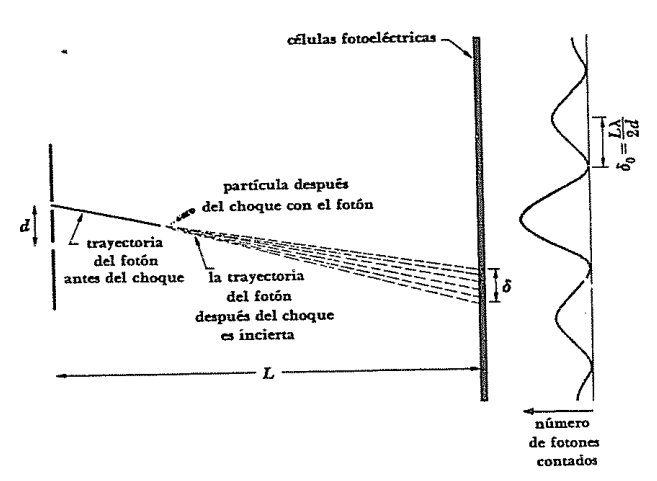
\includegraphics[width = 6.5cm]{../expDualidadOP.png}
    \end{figure}

    \indent Una de las preguntas más difíciles de abordar en física moderna es cómo una partícula puede comportarse tanto como una onda y, en otras circunstancias, como una partícula. A pesar de la existencia de múltiples experimentos que corroboran esta dualidad, la explicación matemática de este fenómeno sigue siendo compleja y no se puede demostrar ambos comportamientos de manera simultánea en un único experimento.\\ 

    \indent Consideremos el experimento ilustrado en la figura al inicio de esta sección. Este muestra un dispositivo experimental en el que la luz, al atravesar una doble rendija, se difracta y los fotones son detectados por una serie de células fotoeléctricas dispuestas sobre una superficie de detección. Los fotones, partículas de luz que también exhiben propiedades ondulatorias, producen un patrón de interferencia característico de ondas al ser registrados por los sensores. Si graficamos el número de fotones detectados por cada sensor en función de su posición en la pantalla, obtenemos un patrón de interferencia, similar al de dos trenes de ondas coherentes.\\

    \begin{figure}[h!]
        \centering
        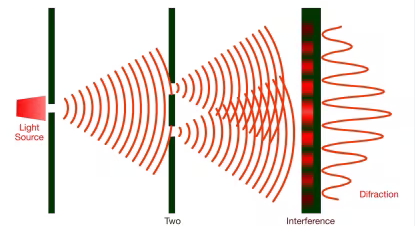
\includegraphics[width = 6.5cm]{../expDOPColor.png}
    \end{figure}

    \indent Este patrón de interferencia persiste incluso cuando la intensidad de la luz es tan baja que, en promedio, solo un fotón pasa a través del aparato en un instante dado. Esto da lugar a cómo puede un único fotón interferir consigo mismo, dicho de otro modo, ¿cómo puede el fotón "sentir" la presencia de ambas rendijas cuando, intuitivamente, solo debería pasar por una? \\

    \indent Abordar este tema conlleva a realizar una modificación en el experimento: Además de las rendijas, se supondrá hay una nube de partículas entre las rendijas y los sensores. Esta nube permite que, al interactuar un fotón con una partícula en su trayecto, podamos determinar cuál de las dos rendijas ha atravesado. Al detectar el fotón, el choque con una de las partículas de la nube le proporciona un impulso detectable, lo que nos permite inferir la trayectoria seguida por el fotón. Sin embargo, al intentar determinar la trayectoria con precisión, la posición del fotón en el eje $y$ estará sujeta a una incertidumbre $\Delta y$.\\

    \indent Si intentamos reducir esta incertidumbre en la coordenada $y$, la incertidumbre en el momento $p_y$ del fotón aumenta debido al principio de incertidumbre de Heisenberg, de acuerdo con la relación:

    \begin{equation}
        \Delta p_y \geq \frac{h}{\Delta y} > \frac{2h}{d}
    \end{equation}

    \indent Donde $d$ es la distancia entre las dos rendijas. Esta relación establece que cuanto más intentemos localizar al fotón (reducir $\Delta y$), mayor será la incertidumbre en su momento $p_y$. \\

    \indent Debido a este incremento en la incertidumbre del momento en el eje $y$, el fotón sufrirá una desviación adicional en su trayectoria. Este cambio en el momento del fotón, $\Delta p_y$, produce una desviación angular en su camino hacia la pantalla de detección, que se puede expresar como:

    \begin{equation}
        \delta = \frac{\Delta p_y}{p_x} L
    \end{equation}

    \indent Donde: \\

      \begin{itemize} [itemsep = -1.5em, topsep = 0em, leftmargin = 1cm]
        \item $p_x$ = momento en la dirección horizontal. \\
        \item $L$ = distancia entre las rendijas y la pantalla de detección. \\
      \end{itemize}

    \indent Este efecto, derivado de la interacción entre el fotón y las partículas en la nube, introduce suficiente alteración en el sistema para destruir el patrón de interferencia característico de ondas. Este resultado es coherente con la interpretación cuántica: cuando intentamos medir con precisión por cuál rendija pasó el fotón (una propiedad de partícula), el comportamiento ondulatorio desaparece.\\

    \indent El experimento ilustra que la naturaleza cuántica de la luz y otras partículas depende de cómo interactuamos con el sistema. Si medimos el fotón como una partícula, obtenemos información sobre su trayectoria pero perdemos el patrón de interferencia ondulatorio. Por otro lado, si no hacemos ninguna medición que interrumpa el sistema, el fotón parece interferir consigo mismo, comportándose como una onda.


\section{MICROSCOPIO ELECTRONICO}

\end{document}


